\subsection{Exercício 4}
No contexto do exercício 4 era necessário criar um modelo de regressão linear simples com o objetivo de determinar o período de "Fidelização" com base na "TarifaMensal" do nosso data frame. Para a criação do modelo, utilizamos a técnica \textbf{hold out} para criação de amostras de treino e de teste. As amostras foram criadas a partir do data frame \textit{Clientes\_DataSet} com proporções de 70\% para treino e 30\% para teste. Uma vez obtidas as amostras de treino e de teste, utilizamos a função \textbf{lm}, em que especificamos que a "Fidelização" depende da "TarifaMensal" através da sintaxe "Fidelização~TarifaMensal" e utilizamos os dados de treino para criação do modelo, dando assim por concluída a alínea a). Para a resolução da alínea b), utilizamos a função \textbf{plot} e \textbf{abline} para criar o respetivo diagrama de dispersão, assim como a sua reta de regressão linear simples, como podemos ver na Fig. \ref{ex_4_b_regressao_simples}. 
\begin{figure}[htbp]
\centerline{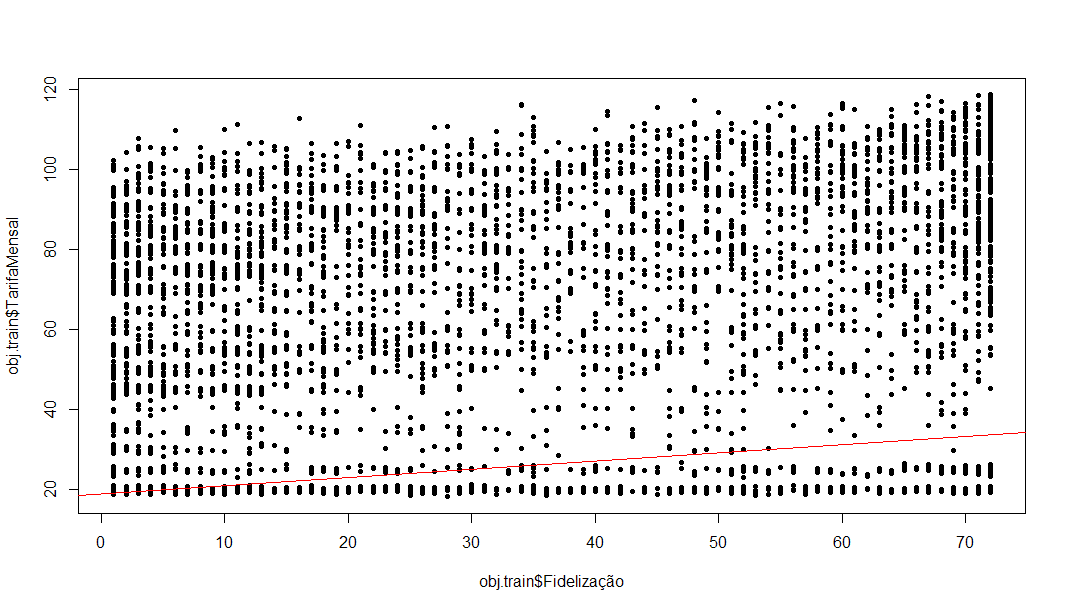
\includegraphics[width=9.5cm]{images/ex_4_b_regressao_simples.png}}
\caption{Visualização do diagrama de dispersão e reta de regressão}
\label{ex_4_b_regressao_simples}
\end{figure}
Para finalizar o exercício 4, na alínea c) era pedido o calculo do erro médio absoluto (MAE) e da raiz quadrada do erro médio (RMSE). Para tal, determinamos a previsão com o modelo de regressão linear previamente criado, utilizando os dados de testes e obtivemos a diferença entre o resultado do nosso modelo, fase ao valor esperado dos dados de teste.Os resultados obtidos foram: 20.48227 para o MAE e 23.48042 para o RMSE.

